\documentclass{beamer}
\usepackage{booktabs}
\newcommand{\fttheory}[1]{\fcolorbox{blue}{blue}{\color{white}\textbf{#1}\hspace{\textwidth}}}
\newcommand{\ftexampl}[1]{\fcolorbox{orange}{orange}{\color{black}\textbf{#1}\hspace{\textwidth}}}
\newcommand{\ftdata}[1]{\fcolorbox{violet}{violet}{\color{white}\textbf{#1}\hspace{\textwidth}}}
\newcommand{\ftheader}[1]{\fcolorbox{lightgray}{lightgray}{\color{black}\textbf{#1}\hspace{\textwidth}}}
\newcommand{\ftvocab}[1]{\fcolorbox{cyan}{cyan}{\color{black}\textbf{#1}\hspace{\textwidth}}}
\newcommand{\usd}{\text{ {\scriptsize USD}}}
\newcommand{\eur}{\text{ {\scriptsize EUR}}}
\newcommand{\aud}{\text{ {\scriptsize AUD}}}
\newcommand{\mxn}{\text{ {\scriptsize MXN}}}
\newcommand{\musd}{\text{ m {\scriptsize USD}}}
\newcommand{\meur}{\text{ m {\scriptsize EUR}}}
\newcommand{\maud}{\text{ m {\scriptsize AUD}}}

\title{Elements of Probability and Statistics}
\begin{document}
\maketitle

\section{Introduction}
\begin{frame}
	\begin{itemize}
		\item Probability and Statistics are not the same
		\item A probability is a number 
		\item E.g. we believe that a coin is heads with probability 0.5 and tails with probability 0.5
		\item A statistic is an \textit{estimation} of a number
		\item E.g. we flip a coin 10 times -- 4 heads, 6 tails
		\item Our estimate is that the coin is heads with probability 0.4 and tails with probability 0.6 
	\end{itemize}
\end{frame}

\begin{frame}{TODO}
	\begin{itemize}
		\item Not going to have students compute statistics from hand. Everything is going to be done via Excel.
		\item However, I think we should bring back all of the Bernoulli statistics. They show up in bond default, binomial option pricing, etc.
	\end{itemize}
\end{frame}

\section{The Normal Distribution}
\begin{frame}{The Normal Distribution}
	\begin{itemize}
		\item Assumption: returns are normally distributed
		\item Consequently, the returns of a \underline{portfolio} are also normally distributed 
		\item The returns of a portfolio are characterized by three attributes of its constituent stocks:
		\begin{enumerate}
			\item the mean return of each stock;
			\item the standard deviation (volatility) of each stock;
			\item the covariance between each pair of stocks.
		\end{enumerate}
		\item We will let $R_{s,t}$ denote the random return of stock $s$ on date $t$
		\item We will focus on monthly returns, although you can just as well think of hourly, daily, weekly, monthly, yearly returns 
	\end{itemize}
\end{frame}

\begin{frame}{The Normal Distribution}
	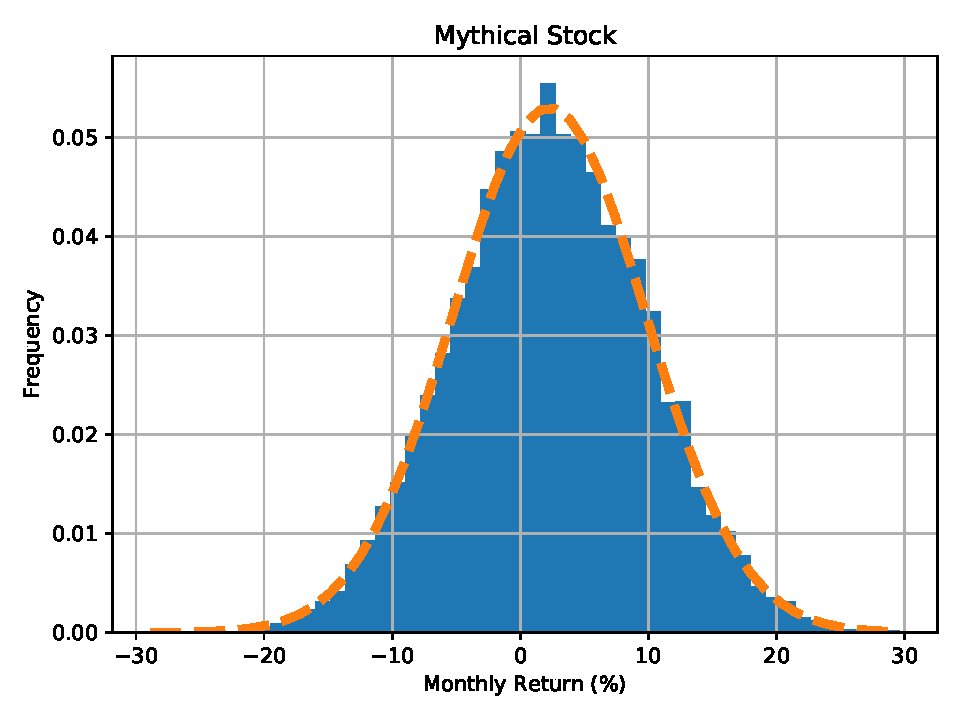
\includegraphics[scale=.55]{myth}
\end{frame}

\begin{frame}{The Normal Distribution}
	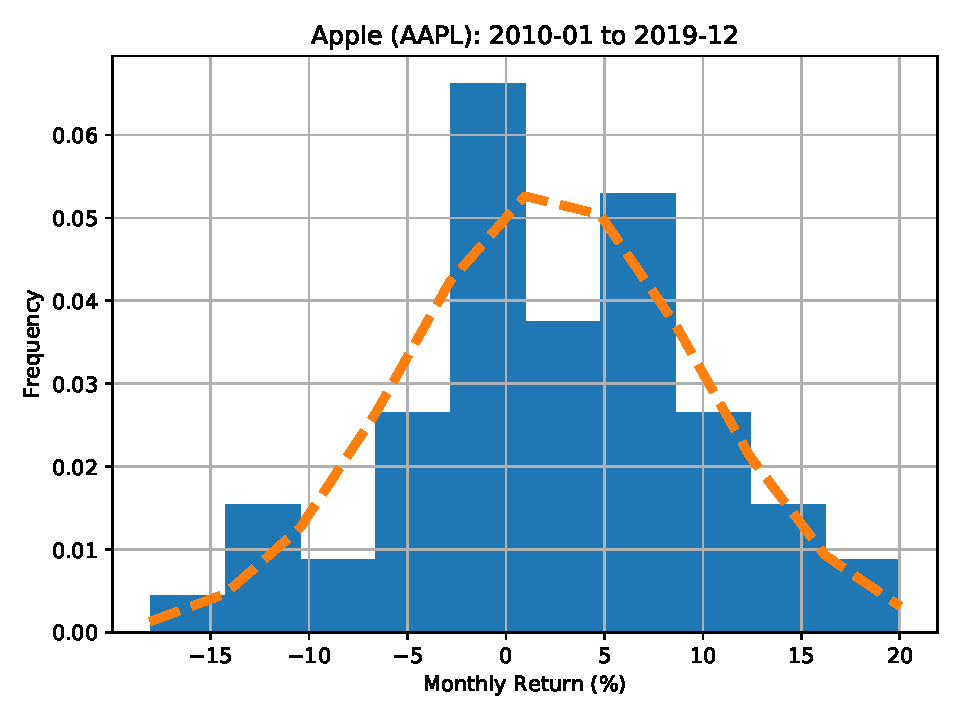
\includegraphics[scale=.55]{apple}
\end{frame}

\section{One Stock}
\begin{frame}{Mean}
	\begin{itemize}
		\item We denoted by $\text{E}[R_{s}]$ the mean, or expectation of $R_{s}$
		\item It is just a \underline{number} 
		\item It tells what the typical return
		\item The mean is expressed in ``\%''
		\item Our \underline{estimate} of the mean return for stock $s$ is
		\begin{equation*}
			\mu_{s}=\frac{1}{N}\sum_{t=1}^{N}{R_{s,t}}
		\end{equation*}
		where $R_{s,t}$ are the \underline{realized} returns
	\end{itemize}
\end{frame}

\begin{frame}{Estimating the Mean}
	What are your estimates of the mean returns for Apple (AAPL) and Home Depot (HD) given the following data?
	\begin{center}
		\begin{tabular}{lll}
\toprule
      date & AAPL return & HD return \\
\midrule
2010-01-01 &      -8.86\% &    -3.18\% \\
2010-02-01 &       6.54\% &    11.39\% \\
2010-03-01 &      14.85\% &     4.44\% \\
\bottomrule
\end{tabular}

	\end{center}
	\pause
	{\color{blue}
	\begin{equation*}
		\mu_{\text{AAPL}}=\frac{-8.86\%+6.54\%+14.85\%}{3}=4.1767\%
	\end{equation*}
	}
	\pause
	{\color{blue}
	\begin{equation*}
		\mu_{\text{HD}}=\frac{-3.18\%+11.39\%+4.44\%}{3}=4.2167\%
	\end{equation*}
	}
\end{frame}

\begin{frame}{Variance}
	\begin{itemize}
		\item We denoted by $\text{Var}[R_{s}]$ the variance of $R_{s}$
		\item The variance is used to construct the standard deviation
		\item The variance does \underline{not} have units
		\item Our \underline{estimate} of the variance of stock $s$ is
		\begin{equation*}
			\sigma_{s}^{2}=\frac{1}{N-1}\sum_{t=1}^{N}{(R_{s,t}-\mu_{s})^{2}}
		\end{equation*}
		\item The ``$N-1$'' makes the estimator unbiased
	\end{itemize}
\end{frame}

\begin{frame}{Estimating the Variance}	
	What is your estimate of the variance of the return for Apple (AAPL) given the data?
	\pause
	{\color{blue}
	We already computed the mean: 4.1767\%. Don't use \% in you calculation! 
	\begin{align*}
		\sigma_{\text{AAPL}}^{2}=\frac{1}{2}&\left[(-0.0886-0.041767)^{2}\right.\\&\left.+(0.0654-0.041767)^{2}\right.\\&\left.+(0.1485-0.041767)^{2}\right]=0.014473
	\end{align*}
	}
\end{frame}
\begin{frame}{Estimating the Variance}	
	What is your estimate of the variance of the return for Home Depot (HD) given the data?
	\pause
	{\color{blue}
	We already computed the mean: 4.2167\%. Don't use \% in you calculation! 
	\begin{align*}
		\sigma_{\text{HD}}^{2}=\frac{1}{2}&\left[(-0.0318-0.042167)^{2}\right.\\&\left.+(0.1139-0.042167)^{2}\right.\\&\left.+(0.0444-0.042167)^{2}\right]=0.005311
	\end{align*}
	}
\end{frame}

\begin{frame}{Standard Deviation}
	\begin{itemize}
		\item We denote by $\text{SD}[R_{s}]$ the standard deviation or \underline{volatility} of $R_{s}$
		\item It is our measure of \underline{risk}
		\item The standard deviation is $\text{SD}[R_{s}]=\sqrt{\text{Var}[R_{s}]}$	
		\item It is expressed in ``\%''
		\pause
		\item {\color{blue}Our \underline{estimate} in the Apple (AAPL) example is $12.0304\%=\sqrt{0.014473}$}
		\item {\color{blue}Our \underline{estimate} in the Home Depot (HD) example is $7.2877\%=\sqrt{0.005311}$}
	\end{itemize}
\end{frame}

\section{Two Stocks}
\begin{frame}
	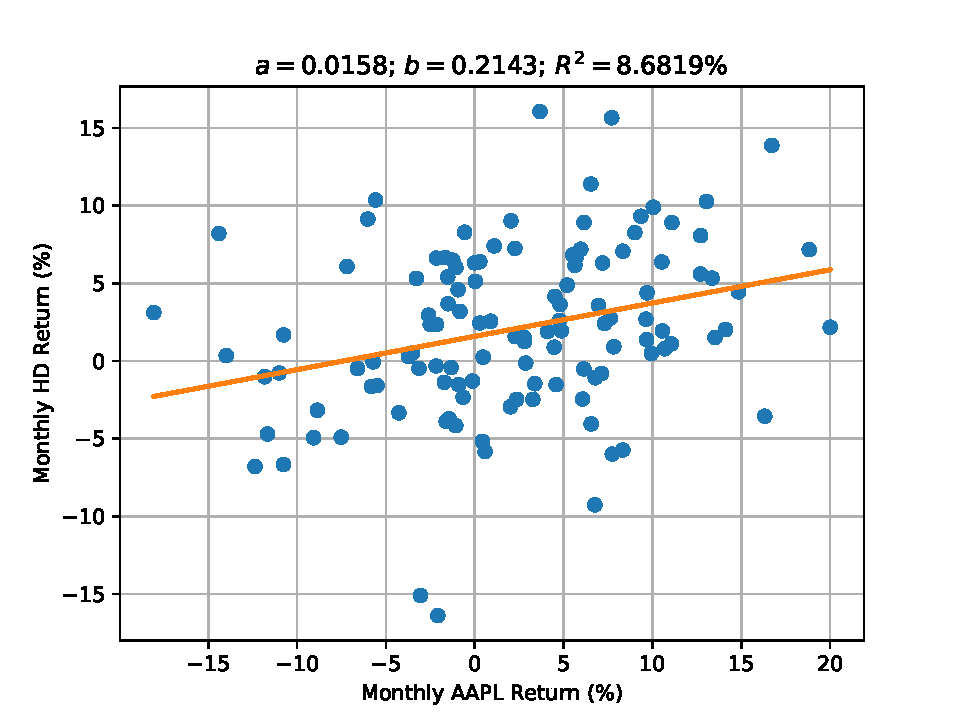
\includegraphics[scale=.55]{aapl_hd}
\end{frame}

\begin{frame}{Covariance}
	\begin{itemize}
		\item Let's think about two stocks, $A$ and $B$	
		\item We denote by $\text{Cov}[R_{A},R_{B}]$ the covariance between the returns on $A$ and $B$
		\item The covariance is used to construct the correlation
		\item The covariance does \underline{not} have units
		\item Our \underline{estimate} of the covariance is 
		\begin{equation*}
			\sigma_{A,B}=\frac{1}{N-1}\sum_{t=1}^{N}{(R_{A,t}-\mu_{A})(R_{B,t}-\mu_{B})}
		\end{equation*}
	\end{itemize}
\end{frame}
\begin{frame}{Estimating the Covariance}
	What is your estimate of the covariance of the returns for Apple and Home Depot given the data?
	\begin{center}
		\begin{tabular}{lll}
\toprule
      date & AAPL return & HD return \\
\midrule
2010-01-01 &      -8.86\% &    -3.18\% \\
2010-02-01 &       6.54\% &    11.39\% \\
2010-03-01 &      14.85\% &     4.44\% \\
\bottomrule
\end{tabular}

	\end{center}
\end{frame}

\begin{frame}{Estimating the Covariance}
	What is your estimate of the covariance of the returns for Apple and Home Depot given the data?
	\pause
	{\color{blue}
	We already computed the mean: 4.1767\%. Don't use \% in you calculation! 
	\begin{align*}
		\sigma_{\text{AAPL,HD}}=\frac{1}{2}&\left[(-0.0886-0.041767)(-0.0318-0.042167)\right.\\
		&\left.+(0.0654-0.041767)(0.1139-0.042167)\right.\\
		&\left.+(0.1485-0.041767)(0.0444-0.042167)\right]\\
		&=0.005788
	\end{align*}
	}
\end{frame}

\begin{frame}{Correlation}
	\begin{itemize}
		\item We denote by $\text{Corr}[R_{A},R_{B}]$ the correlation between the returns of $A$ and $B$
		\item It is given by
			\begin{equation*}
				\text{Corr}[R_{A},R_{B}]=\frac{\text{Cov}[R_{A},R_{B}]}{\text{SD}[R_{A}]\text{SD}[R_{B}]}
			\end{equation*}
	\end{itemize}
\pause
	{\color{blue}
		 Our estimate in the Apple, Home Depot example is
			\begin{align*}
				\text{Corr}[R_{AAPL},R_{HD}]&=\frac{\text{Cov}[R_{AAPL},R_{HD}]}{\text{SD}[R_{AAPL}]\text{SD}[R_{HD}]}\\
				&=\frac{0.005788}{.0120304\times 0.072877}=0.6602
			\end{align*}
}
\end{frame}

\begin{frame}{Correlation}
		The correlation is between $-1$ and $+1$, with a correlation of $-1$ meaning perfectly negatively correlated ($A$ goes up, $B$ goes down), a correlation of $0$ meaning they are not correlated at all ($A$'s return doesn't tell us anything about $B$'s return), and a correlation of $+1$ meaning perfectly positively correlated ($A$ goes up, $B$ goes up) 
\end{frame}

\section{Portfolio}
\begin{frame}{Portfolio of Two Stocks}
	\begin{itemize}
		\item We are going to focus on portfolios with two stocks
		\item All of the computations that follow can be done with an arbitrary number of stocks --- we just need some linear algebra 	
		\item Consider a portfolio with $x_{A}$ in stock $A$ and $x_{B}$ in stock $B$
		\item $x_{A}$ and $x_{B}$ must sum to one: $x_{A}+x_{B}=1$
		\item $x>1$ means we are borrowing (or financing with short)
		\item $x<0$ means we are shorting
		\item The random return of the portfolio is
		\begin{equation*}
			R_{P}=x_{A}R_{A}+x_{B}R_{B}
		\end{equation*}
	\end{itemize}
\end{frame}

\begin{frame}{Mean and Volatility}
	\begin{itemize}
		\item The mean return of the portfolio is
		\begin{equation*}
			\text{E}[R_{P}]=x_{A}\text{E}[R_{A}]+x_{B}\text{E}[R_{B}]
		\end{equation*}
		\item The variance of the portfolio is
		\begin{equation*}
			\text{Var}[R_{P}]=x_{A}^{2}\text{Var}[R_{A}]+x_{B}^{2}\text{Var}[R_{B}]+2x_{A}x_{B}\text{Cov}[R_{A},R_{B}]
		\end{equation*}
		\item Therefore, the volatility of the portfolio is
		\begin{equation*}
			\text{SD}[R_{P}]=\sqrt{\text{Var}[R_{P}]}
		\end{equation*}
	\end{itemize}
\end{frame}
\begin{frame}{Mean and Volatility}
	What is the mean return and volatility of a portfolio that is 25\% in Apple (AAPL) and 75\% in Home Depot (HD)?
	\pause
	{\color{blue}
	The mean return is
	\begin{equation*}
		\mu_{P}=.25\times(4.1767\%)+.75\times(4.2167\%)=4.2067\%
	\end{equation*}
	}
	{\color{blue}
	The variance is
	\begin{align*}
		\sigma_{P}^{2}&=(.25)^2(0.014473)+(.75)^2(0.005311)+2(.25)(.75)(0.005788)\\
		&=0.006063
	\end{align*}
	and hence the volatlity is
	\begin{equation}
		\sigma_{P}=\sqrt{0.006063}=7.7862\%
	\end{equation}
	}
\end{frame}

\section{Regression}

\begin{frame}{Intercept and Slope}
	\begin{itemize}
		\item Suppose that we regress the returns of stock $B$ on the returns of stock $A$ (the ordering is important)
		\item Put differently, $A$ is our x-axis and $B$ is our y-axis	
		\item We want to choose $a$ and $b$ to ``fit'' the equation 
		\begin{equation}
			R_{B}=a+bR_{A}
		\end{equation}
		to the data
		\item The estimates for $a$ and $b$ are
		\begin{align*}	
			\hat{b}&=\frac{\text{Cov}[R_{A},R_{B}]}{\text{Var}[R_{A}]}=\frac{\text{SD}[R_{B}]}{\text{SD}[R_{A}]}\text{Corr}[R_{A},R_{B}]\\
			\hat{a}&=\text{E}[R_{B}]-\hat{b}\text{E}[R_{A}]
		\end{align*}
	\end{itemize}
\end{frame}

\begin{frame}{R-Squared}
	\begin{itemize}
		\item The \emph{R-squared} (written as $R^{2}$) is a measure of the ``goodness-of-fit'' 
		\item It is the ratio of the variance in the data that can be explained by the regression line to the total variance in the data:
			\begin{equation}
				R^{2}=\frac{b^{2}\text{Var}[R_{A}]}{\text{Var}[R_{B}]}=\text{Corr}[R_{P}]^{2}
			\end{equation}
		\item This is only true with a slope and an intercept; $R^{2}$ is a bit more complicated in more general regresssions
		\item It \underline{can} be written in terms of \%
		\item An $R^{2}$ of 100\% means the regression perfectly fits the data.
	\end{itemize}
\end{frame}

\begin{frame}{Apple and MSFT}
	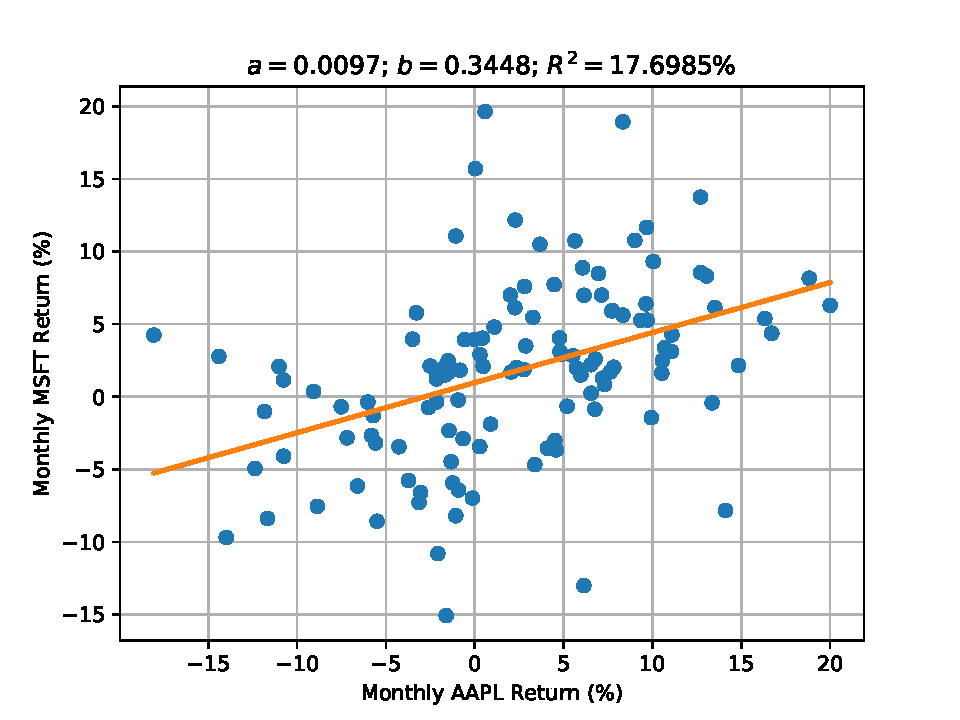
\includegraphics[scale=.55]{aapl_msft}
\end{frame}

\begin{frame}{Apple and P\&G}
	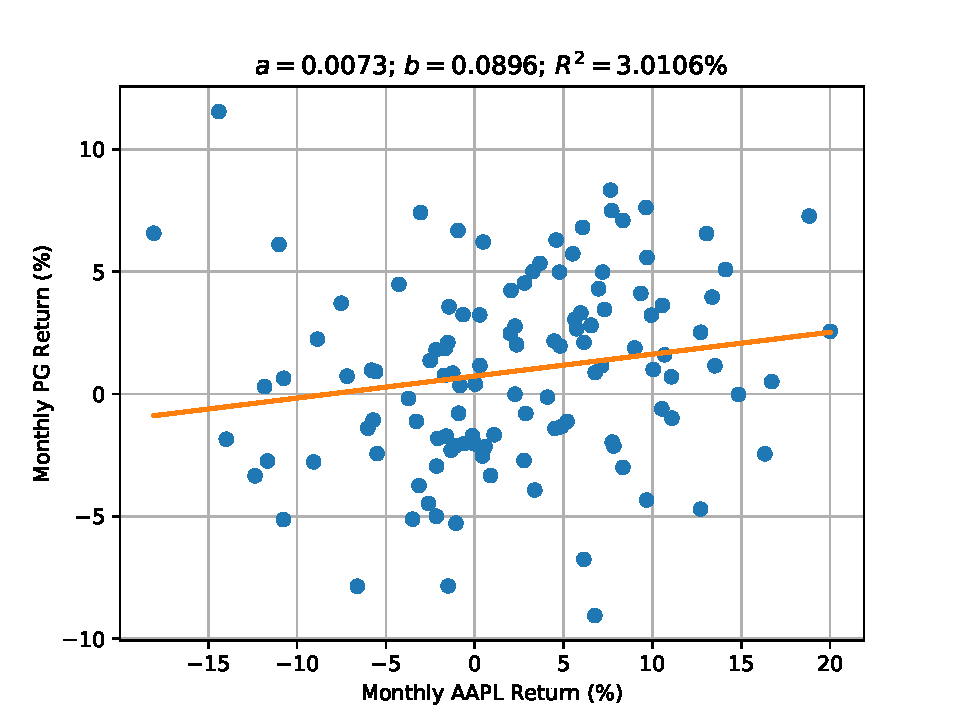
\includegraphics[scale=.55]{aapl_pg}
\end{frame}

\begin{frame}{Example}
	Consider American Express (AXP) and Visa (V). Suppose that we regress Visa's returns on those of American Express.  $\text{E}[R_{\text{AXP}}]=1.2100\%$ $\text{E}[R_{\text{V}}]=1.9960\%$, $\text{SD}[R_{\text{AXP}}]=5.7304\%$ $\text{SD}[R_{\text{V}}]=5.0389\%$, $\text{Corr}[R_{\text{AXP}}]=0.5150$
	\pause
	{\color{blue}
	\begin{align*}	
		\hat{b}&=\frac{5.0389\%}{5.7304\%}\times0.5150=0.4529\\
		\hat{a}&=1.9960\%-0.4529\times1.2100\%=1.4480\%\\
		R^{2}&=(0.5150)^2=26.5225\%
	\end{align*}
	}
\end{frame}

\end{document}
